\begin{frame}{What is a Brownian motion?}

\begin{figure}
		\centering
		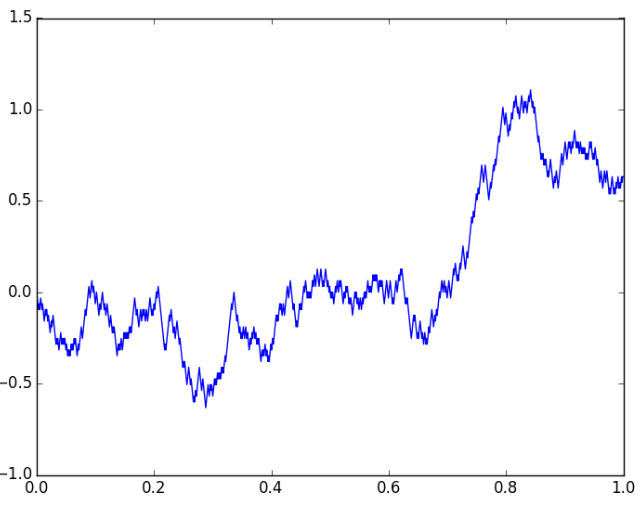
\includegraphics[width=300]{Images/BrownianMotion.png}
\end{figure}
\FloatBarrier

\pause
A stochastic process $t \longmapsto W_t$ is a Brownian motion if: 

\begin{itemize}
	\item $W_0 = 0$
	\pause
	\item $W_t$ has independent increments
	\pause
	\item $W_t - W_s$ is $\textbf{N}(0, t-s)$, a gaussian random variable with mean 0 and variance $t-s$.
\end{itemize}
	
\end{frame}


\begin{frame}{How to generate one Brownian motion?}

We need:

\bigskip

\begin{itemize}
	\item a time horizon, for example 1 year;
	\pause
	\bigskip
	\item a number of time steps, for example 10;
	\pause
	\bigskip
	\item a number of simulations, for example 100;
	\pause
	\bigskip
	\item a discretization of the Brownian motion:
		\begin{displaymath}
			W_{t+\Delta t} = W_t + \sigma \cdot \sqrt{\Delta t} \cdot Z,
		\end{displaymath}
		\pause
		where $Z$ is $\textbf{N}(0,1)$ and $\sigma>0$ is a volatility factor.
\end{itemize}



\end{frame}


\begin{frame}{Two correlated Brownian motions - 1}

	\begin{figure}
		\centering
		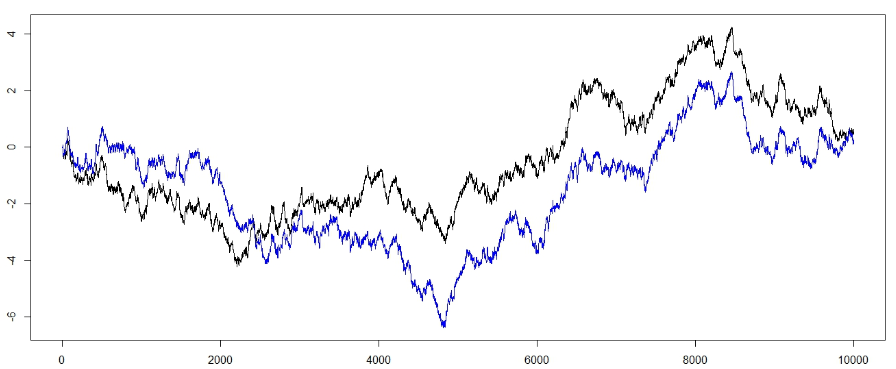
\includegraphics[width=400]{Images/CorrelatedBrownianMotions.png}
	\end{figure}

\pause
	\begin{displaymath}
		W^1_{t+\Delta t} & = W^1_t + \sigma_1 \cdot \sqrt{\Delta t} \cdot Z_1
	\end{displaymath}
	\pause
	\begin{displaymath}
		W^2_{t+\Delta t} & = W^2_t + \sigma_2 \cdot \sqrt{\Delta t} \cdot Z_2 
	\end{displaymath}

	where
		\pause
	\begin{displaymath}
		Z_2 & = \rho \cdot Z_1 + \sqrt{1 - \rho^2} \cdot X_1
	\end{displaymath}
	\pause
	and $Z_1$, $X_1$ are independent $\textbf{N}(0,1)$, $\rho\in[-1 ,1]$.

\end{frame}


\begin{frame}{Two correlated Brownian motions - 2}
	In matrix notation:
	
	\pause
	\begin{displaymath}
		\begin{bmatrix}
			Z_1 \\
			Z_2
		\end{bmatrix}
		=
		\underbrace{\begin{bmatrix}
			1 & 0 \\
			\rho & \sqrt{1-\rho^2}
		\end{bmatrix}}_{C}
		\cdot
		\begin{bmatrix}
			Z_1 \\
			X_1
		\end{bmatrix}
	\end{displaymath}
	
	\pause
	Observe:
	
	\begin{align*}
		C \cdot C^{T} & = 
		\underbrace{\begin{bmatrix}
			1 & \rho \\
			\rho & 1
		\end{bmatrix}}_{Cov} \\
		& = \begin{bmatrix}
			Var(Z_1) & Cov(Z_1, Z_2) \\
			Cov(Z_1, Z_2) & Var(Z_2)
		\end{bmatrix}
	\end{align*}
	
	\pause
	$Cov$ is the Variance-Covariance matrix.
	
\end{frame}


\begin{frame}{Many correlated Brownian motions - 1}

\pause
We have $Z_1, Z_2, \ldots, Z_N$ all correlated to each other. 

\pause
\bigskip
How do we generate $N$ correlated random variables?

\pause
\bigskip
$\Rightarrow$ Cholesky decomposition

\pause
\begin{displaymath}
	C \cdot C^{T} = 
		\begin{bmatrix}
			1 & \rho_{12} & \ldots & \rho_{1N} \\
			\rho_{12} & 1 & & \vdots \\
			\vdots & \vdots & & \vdots\\
			\rho_{1N} & \rho_{2N} & \dots & 1
		\end{bmatrix}
\end{displaymath}

where C is a lower triangular matrix.

\end{frame}


\begin{frame}{Many correlated Brownian motions - 2}

In matrix notation:

\pause
\begin{displaymath}
	\begin{bmatrix}
			Z_1 \\
			Z_2 \\
			\vdots \\
			Z_N
		\end{bmatrix} 
		= C \cdot 
		\begin{bmatrix}
			Z_1 \\
			X_1 \\
			\vdots \\
			X_{N-1}
		\end{bmatrix} 
\end{displaymath}

\bigskip
and $Z_1, X_1, \ldots, X_{N-1}$ are independent $\textbf{N}(0,1)$.

\pause
\bigskip
Eventually:
\begin{align*}
		W^1_{t+\Delta t} & = W^1_t + \sigma_1 \cdot \sqrt{\Delta t} \cdot Z_1 \\
	\vdots & \\
	W^N_{t+\Delta t} & = W^N_t + \sigma_N \cdot \sqrt{\Delta t} \cdot Z_N \\
\end{align*}

\end{frame}